% !TeX root = ../main.tex
% Add the above to each chapter to make compiling the PDF easier in some editors.


\chapter{Background}\label{ch:background}

In this chapter we will discuss the technical background required for the later sections.
We will describe the architecture of MCTOLL in \cref{sec:mctoll} and its limitations in \cref{subsec:limitations}.


\section{Control Flow Graph}\label{sec:cfg}

A \gls{CFG}~\parencite{cfg} is a graph representation of a program where the nodes represent basic blocks, while edges represent jumps.

\paragraph{Basic Blocks}
A basic block is a segment of code without any jumps or jump targets where jump targets start a block while jumps end a block.
\Cref{fig:cfg} is an example \gls{CFG} with an entry node (1), an exit node (6) and a loop (nodes 2, 3, 4, 5).

\begin{figure}[htpb]
    \centering
    \begin{tikzpicture}[shorten >=1pt,node distance=2cm,on grid,auto]
        \node[state] (bb0) {1};
        \node[state] (bb1) [below=of bb0] {2};
        \node[state] (bb2) [below left=of bb1] {3};
        \node[state] (bb3) [below=of bb1] {4};
        \node[state] (bb4) [below=of bb3] {5};
        \node[state] (bb5) [below right=of bb1] {6};
        \path[->]
            (bb0) edge (bb1)
            (bb1) edge (bb2)
            (bb1) edge (bb3)
            (bb1) edge (bb5)
            (bb2) edge (bb4)
            (bb3) edge (bb4)
            (bb4) edge [bend right=30] (bb1)
        ;
    \end{tikzpicture}
    \caption{Example of a control flow graph}
    \label{fig:cfg}
\end{figure}

\subsection{Dominator Trees}\label{subsec:dominator-trees}

In a \gls{CFG} a node $n$ dominates a node $p$ if every path from the entry node to $p$ must go through $n$~\parencite{10.1145/1460299.1460314}.

Additionally, the following definitions hold:
\begin{itemize}
    \item A node $n$ \textit{strictly dominates} a node $p$ if $n$ dominates $p$ and $n \neq p$.
    \item A node $n$ \textit{immediately dominates} a node $p$ if $n$ strictly dominates $p$ but there exists no node $n'$ that strictly dominates $p$.
    \item A dominator tree is a directed graph where the children of a node $n$ are the nodes that $n$ immediately dominates.
\end{itemize}

Dominator trees can be derived from \gls{CFG}s as shown by \citeauthor{10.1145/362835.362838} in \cite{10.1145/362835.362838}.

\begin{figure}[htpb]
    \centering
    \begin{tikzpicture}
        [shorten >=1pt,node distance=2cm,on grid,auto]
        \node[state] (bb0) {1};
        \node[state] (bb1) [below=of bb0] {2};
        \node[state] (bb2) [below left=1.5cm and 3cm of bb1] {3};
        \node[state] (bb3) [below left=1.5cm and 1cm of bb1] {4};
        \node[state] (bb4) [below right=1.5cm and 1cm of bb1] {5};
        \node[state] (bb5) [below right=1.5cm and 3cm of bb1] {6};
        \path[->]
        (bb0) edge (bb1)
        (bb1) edge (bb2)
        (bb1) edge (bb3)
        (bb1) edge (bb4)
        (bb1) edge (bb5)
        ;
    \end{tikzpicture}
    \label{fig:dominator-tree}
    \caption{Dominator tree from the \gls{CFG} in \cref{fig:cfg}}
\end{figure}


\section{LLVM}\label{sec:llvm}

LLVM is a set of compiler and toolchain technologies, designed around an \gls{IR}~\parencite{llvm}.
LLVM was started as a research project at the University of Illinois.
The \gls{IR} serves as a portable high-level assembly language, which can be targeted by compiler frontends such as clang\footnote{\url{https://clang.llvm.org}}, rustc\footnote{\url{https://www.rust-lang.org}}, swiftc\footnote{\url{https://swift.org}}, and others.
LLVM transforms and optimizes the intermediate representation with a set of compiler passes before passing it on to LLVM's codegen, which compiles the IR to the target's machine code~\parencite{LLVM_CGO04}.

\begin{figure}[htpb]
    \begin{equation}
        \mathbb{P}_{\mathsf{C}}
        \xrightarrow{\mathsf{clang}} \mathbb{P}_\mathsf{IR}
        \xrightarrow{\mathsf{LLVM.opt}} \mathbb{P}_\mathsf{IR}'
        \xrightarrow{\mathsf{LLVM.codegen}} \mathbb{P}_\mathsf{target}
    \end{equation}
    \label{fig:llvm-clang-workflow}
    \caption{Workflow of clang and LLVM}
\end{figure}

\subsection{LLVM Intermediate Representation}\label{subsec:llvm-intermediate-representation}

LLVM \gls{IR} is in \gls{SSA} form, used by many intermediate languages to simplify compiler optimizations.
\gls{SSA} is a property of a language which requires that each variable is assigned exactly once and defined before it is used by subsequent instructions.
Constant propagation, dead code elimination, and register allocation are some compiler optimizations that are enabled by the \gls{SSA} form~\parencite{ssa}.

In LLVM IR, each expression needs to be type-annotated. LLVM natively supports arbitrary-sized integers, pointers, tuples, single- and double-precision floating-point numbers, and vectors.
These type annotations allow LLVM to perform some optimizations that would not be possible with a traditional three-address code.

\begin{lstlisting}[label={lst:llvm-ir},caption={Example of LLVM IR addding 5 + 2},captionpos=b]
    %0 = i32 5
    %1 = add i32 %0, i32 2
\end{lstlisting}

\subsection{Intrinsic Functions}

Intrinsic functions (or built-in functions) are functions that are available for use by the programmer but implemented in the compiler itself.
Depending on the target, the compiler may insert a series of instructions in place of the function call or call a function in some library.
This behaviour is opaque to the user.

In LLVM some essential operations such as addition with overflow or square roots are implemented as intrinsic functions.
On platforms such as x86, these are then compiled to a single CPU instruction, while they might be implemented in software on other platforms.


\section{x86\_64}\label{sec:x86-64}

x86\_64 is an extension to x86 designed by AMD and used by the main desktop chip manufacturers Intel and AMD.
x86\_64 is a \gls{CISC} architecture that builds on x86 in a backwards-compatible way, supporting all 32 bit instructions while adding an array of features.
The most important ones are the expansion of general purpose registers to 64 bits (see \cref{fig:x86-64-rax-subregs}), the addition of new general purpose registers and the possibility to address an extended 64 bit address space.

\begin{figure}[htpb]
    \centering
    \resizebox{\textwidth}{!}{
        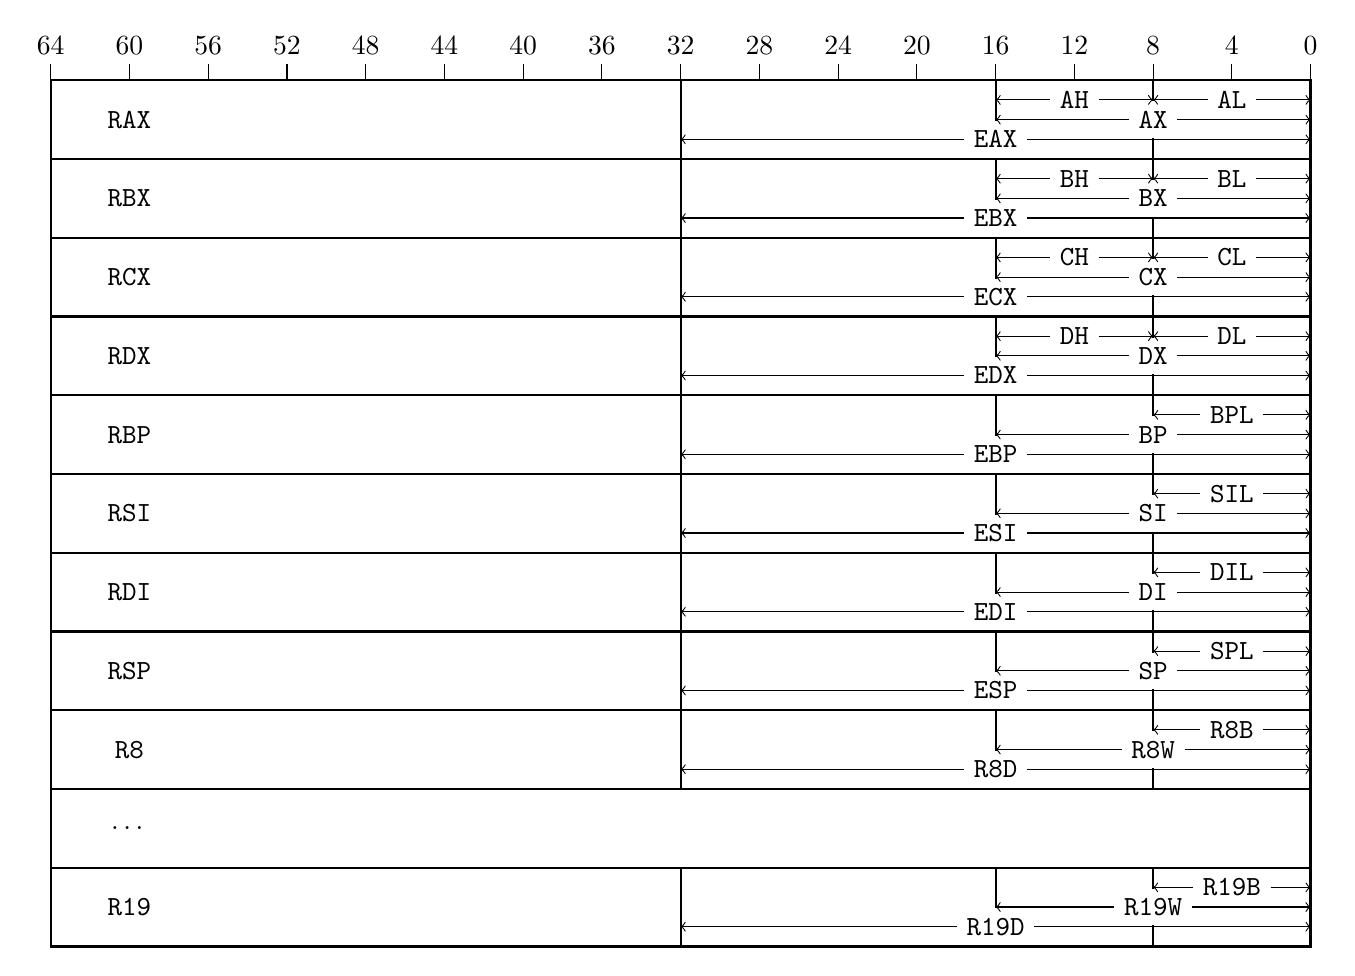
\begin{tikzpicture}
            \tikzset{every edge quotes/.style =
                    { fill = white,
                sloped  }}
            \foreach \x in {0,...,16} {
                \draw (\x,12) -- (\x,12.2);
                \pgfmathsetmacro\display{64-\x*4}
                \node [above] at (\x,12.2) {\pgfmathprintnumber{\display}};
            }

            % generated with python pls don't judge me
% RAX
            \draw[thick] (0,11) rectangle (16,12) node[pos=.5] {};
            \path (1,11) -- node (RAX) {\texttt{RAX}} (1,12);

            \path (14,11.75) -- node (AL) {\texttt{AL}} (16,11.75);
            \draw[<-] (14,11.75) -- (AL);
            \draw[->] (AL) -- (16,11.75);
            \path (12,11.75) -- node (AH) {\texttt{AH}} (14,11.75);
            \draw[<-] (12,11.75) -- (AH);
            \draw[->] (AH) -- (14,11.75);
            \path (12,11.5) -- node (AX) {\texttt{AX}} (16,11.5);
            \draw[<-] (12,11.5) -- (AX);
            \draw[->] (AX) -- (16,11.5);
            \path (8,11.25) -- node (EAX) {\texttt{EAX}} (16,11.25);
            \draw[<-] (8,11.25) -- (EAX);
            \draw[->] (EAX) -- (16,11.25);

            \draw[thick] (8,11) -- (8,12);
            \draw[thick] (12,12) -- (EAX);
            \draw[thick] (14,12) -- (AX);
            \draw[thick] (AX) -- (14,11);
% RBX
            \draw[thick] (0,10) rectangle (16,11) node[pos=.5] {};
            \path (1,10) -- node (RBX) {\texttt{RBX}} (1,11);

            \path (14,10.75) -- node (BL) {\texttt{BL}} (16,10.75);
            \draw[<-] (14,10.75) -- (BL);
            \draw[->] (BL) -- (16,10.75);
            \path (12,10.75) -- node (BH) {\texttt{BH}} (14,10.75);
            \draw[<-] (12,10.75) -- (BH);
            \draw[->] (BH) -- (14,10.75);
            \path (12,10.5) -- node (BX) {\texttt{BX}} (16,10.5);
            \draw[<-] (12,10.5) -- (BX);
            \draw[->] (BX) -- (16,10.5);
            \path (8,10.25) -- node (EBX) {\texttt{EBX}} (16,10.25);
            \draw[<-] (8,10.25) -- (EBX);
            \draw[->] (EBX) -- (16,10.25);

            \draw[thick] (8,10) -- (8,11);
            \draw[thick] (12,11) -- (EBX);
            \draw[thick] (14,11) -- (BX);
            \draw[thick] (BX) -- (14,10);
% RCX
            \draw[thick] (0,9) rectangle (16,10) node[pos=.5] {};
            \path (1,9) -- node (RCX) {\texttt{RCX}} (1,10);

            \path (14,9.75) -- node (CL) {\texttt{CL}} (16,9.75);
            \draw[<-] (14,9.75) -- (CL);
            \draw[->] (CL) -- (16,9.75);
            \path (12,9.75) -- node (CH) {\texttt{CH}} (14,9.75);
            \draw[<-] (12,9.75) -- (CH);
            \draw[->] (CH) -- (14,9.75);
            \path (12,9.5) -- node (CX) {\texttt{CX}} (16,9.5);
            \draw[<-] (12,9.5) -- (CX);
            \draw[->] (CX) -- (16,9.5);
            \path (8,9.25) -- node (ECX) {\texttt{ECX}} (16,9.25);
            \draw[<-] (8,9.25) -- (ECX);
            \draw[->] (ECX) -- (16,9.25);

            \draw[thick] (8,9) -- (8,10);
            \draw[thick] (12,10) -- (ECX);
            \draw[thick] (14,10) -- (CX);
            \draw[thick] (CX) -- (14,9);
% RDX
            \draw[thick] (0,8) rectangle (16,9) node[pos=.5] {};
            \path (1,8) -- node (RDX) {\texttt{RDX}} (1,9);

            \path (14,8.75) -- node (DL) {\texttt{DL}} (16,8.75);
            \draw[<-] (14,8.75) -- (DL);
            \draw[->] (DL) -- (16,8.75);
            \path (12,8.75) -- node (DH) {\texttt{DH}} (14,8.75);
            \draw[<-] (12,8.75) -- (DH);
            \draw[->] (DH) -- (14,8.75);
            \path (12,8.5) -- node (DX) {\texttt{DX}} (16,8.5);
            \draw[<-] (12,8.5) -- (DX);
            \draw[->] (DX) -- (16,8.5);
            \path (8,8.25) -- node (EDX) {\texttt{EDX}} (16,8.25);
            \draw[<-] (8,8.25) -- (EDX);
            \draw[->] (EDX) -- (16,8.25);

            \draw[thick] (8,8) -- (8,9);
            \draw[thick] (12,9) -- (EDX);
            \draw[thick] (14,9) -- (DX);
            \draw[thick] (DX) -- (14,8);
% RBP
            \draw[thick] (0,7) rectangle (16,8) node[pos=.5] {};
            \path (1,7) -- node (RBP) {\texttt{RBP}} (1,8);

            \path (14,7.75) -- node (BPL) {\texttt{BPL}} (16,7.75);
            \draw[<-] (14,7.75) -- (BPL);
            \draw[->] (BPL) -- (16,7.75);
            \path (12,7.5) -- node (BP) {\texttt{BP}} (16,7.5);
            \draw[<-] (12,7.5) -- (BP);
            \draw[->] (BP) -- (16,7.5);
            \path (8,7.25) -- node (EBP) {\texttt{EBP}} (16,7.25);
            \draw[<-] (8,7.25) -- (EBP);
            \draw[->] (EBP) -- (16,7.25);

            \draw[thick] (8,7) -- (8,8);
            \draw[thick] (12,8) -- (EBP);
            \draw[thick] (14,8) -- (BP);
            \draw[thick] (BP) -- (14,7);
% RSI
            \draw[thick] (0,6) rectangle (16,7) node[pos=.5] {};
            \path (1,6) -- node (RSI) {\texttt{RSI}} (1,7);

            \path (14,6.75) -- node (SIL) {\texttt{SIL}} (16,6.75);
            \draw[<-] (14,6.75) -- (SIL);
            \draw[->] (SIL) -- (16,6.75);
            \path (12,6.5) -- node (SI) {\texttt{SI}} (16,6.5);
            \draw[<-] (12,6.5) -- (SI);
            \draw[->] (SI) -- (16,6.5);
            \path (8,6.25) -- node (ESI) {\texttt{ESI}} (16,6.25);
            \draw[<-] (8,6.25) -- (ESI);
            \draw[->] (ESI) -- (16,6.25);

            \draw[thick] (8,6) -- (8,7);
            \draw[thick] (12,7) -- (ESI);
            \draw[thick] (14,7) -- (SI);
            \draw[thick] (SI) -- (14,6);
% RDI
            \draw[thick] (0,5) rectangle (16,6) node[pos=.5] {};
            \path (1,5) -- node (RDI) {\texttt{RDI}} (1,6);

            \path (14,5.75) -- node (DIL) {\texttt{DIL}} (16,5.75);
            \draw[<-] (14,5.75) -- (DIL);
            \draw[->] (DIL) -- (16,5.75);
            \path (12,5.5) -- node (DI) {\texttt{DI}} (16,5.5);
            \draw[<-] (12,5.5) -- (DI);
            \draw[->] (DI) -- (16,5.5);
            \path (8,5.25) -- node (EDI) {\texttt{EDI}} (16,5.25);
            \draw[<-] (8,5.25) -- (EDI);
            \draw[->] (EDI) -- (16,5.25);

            \draw[thick] (8,5) -- (8,6);
            \draw[thick] (12,6) -- (EDI);
            \draw[thick] (14,6) -- (DI);
            \draw[thick] (DI) -- (14,5);
% RSP
            \draw[thick] (0,4) rectangle (16,5) node[pos=.5] {};
            \path (1,4) -- node (RSP) {\texttt{RSP}} (1,5);

            \path (14,4.75) -- node (SPL) {\texttt{SPL}} (16,4.75);
            \draw[<-] (14,4.75) -- (SPL);
            \draw[->] (SPL) -- (16,4.75);
            \path (12,4.5) -- node (SP) {\texttt{SP}} (16,4.5);
            \draw[<-] (12,4.5) -- (SP);
            \draw[->] (SP) -- (16,4.5);
            \path (8,4.25) -- node (ESP) {\texttt{ESP}} (16,4.25);
            \draw[<-] (8,4.25) -- (ESP);
            \draw[->] (ESP) -- (16,4.25);

            \draw[thick] (8,4) -- (8,5);
            \draw[thick] (12,5) -- (ESP);
            \draw[thick] (14,5) -- (SP);
            \draw[thick] (SP) -- (14,4);
% R8
            \draw[thick] (0,3) rectangle (16,4) node[pos=.5] {};
            \path (1,3) -- node (R8) {\texttt{R8}} (1,4);

            \path (14,3.75) -- node (R8B) {\texttt{R8B}} (16,3.75);
            \draw[<-] (14,3.75) -- (R8B);
            \draw[->] (R8B) -- (16,3.75);
            \path (12,3.5) -- node (R8W) {\texttt{R8W}} (16,3.5);
            \draw[<-] (12,3.5) -- (R8W);
            \draw[->] (R8W) -- (16,3.5);
            \path (8,3.25) -- node (R8D) {\texttt{R8D}} (16,3.25);
            \draw[<-] (8,3.25) -- (R8D);
            \draw[->] (R8D) -- (16,3.25);

            \draw[thick] (8,3) -- (8,4);
            \draw[thick] (12,4) -- (R8D);
            \draw[thick] (14,4) -- (R8W);
            \draw[thick] (R8W) -- (14,3);
%
            \draw[thick] (0,2) rectangle (16,3) node[pos=.5] {};
            \path (1,2) -- node (dots) {\dots} (1,3);

% R19
            \draw[thick] (0,1) rectangle (16,2) node[pos=.5] {};
            \path (1,1) -- node (R19) {\texttt{R19}} (1,2);

            \path (14,1.75) -- node (R19B) {\texttt{R19B}} (16,1.75);
            \draw[<-] (14,1.75) -- (R19B);
            \draw[->] (R19B) -- (16,1.75);
            \path (12,1.5) -- node (R19W) {\texttt{R19W}} (16,1.5);
            \draw[<-] (12,1.5) -- (R19W);
            \draw[->] (R19W) -- (16,1.5);
            \path (8,1.25) -- node (R19D) {\texttt{R19D}} (16,1.25);
            \draw[<-] (8,1.25) -- (R19D);
            \draw[->] (R19D) -- (16,1.25);

            \draw[thick] (8,1) -- (8,2);
            \draw[thick] (12,2) -- (R19D);
            \draw[thick] (14,2) -- (R19W);
            \draw[thick] (R19W) -- (14,1);
        \end{tikzpicture}
    }
    \caption{x86\_64 general purpose registers}
    \label{fig:x86-64-rax-subregs}
\end{figure}

\subsection{SSE}

Most modern CPUs feature some kind of \gls{SIMD} instructions and registers.
The most widely used \gls{SIMD} extension for x86 is SSE (Streaming SIMD Extensions).
Additionally, SSE is also utilized to perform floating-point operations.
It uses the independent \texttt{XMM} registers (see \cref{fig:vector-regs}).

\begin{figure}[htpb]
    \centering
    \resizebox{\textwidth}{!}{
        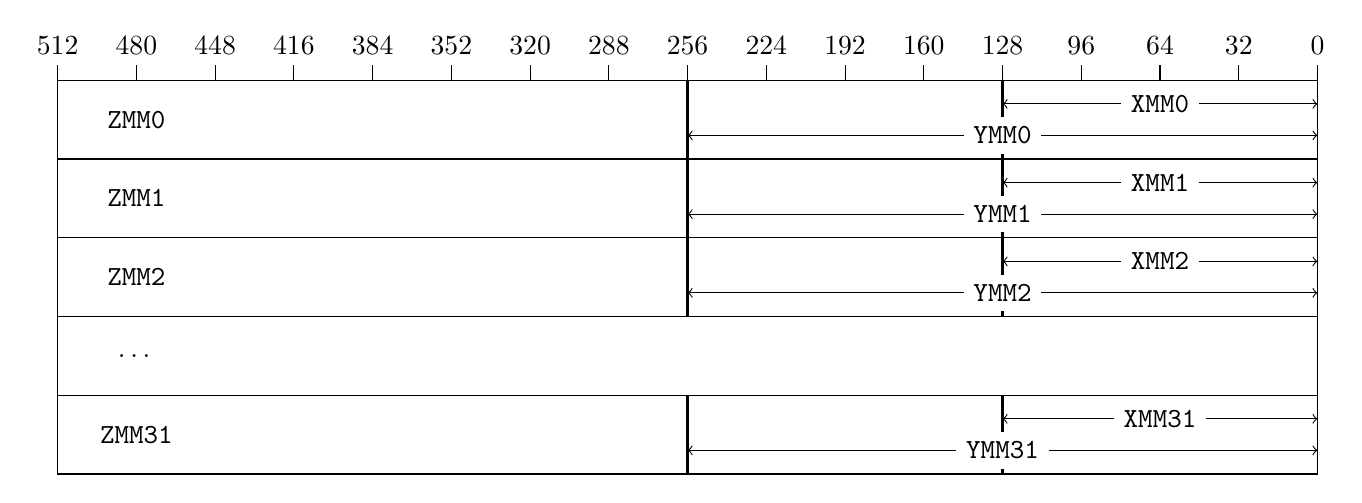
\begin{tikzpicture}
            \foreach \x in {0,...,16} {
                \draw (\x,5) -- (\x,5.2);
                \pgfmathsetmacro\display{512-\x*32}
                \node [above] at (\x,5.2) {\pgfmathprintnumber{\display}};
            }
            % MM0
            \draw (0,4) rectangle (16,5) node[pos=.5] {};
            \path (1,4) -- node (ZMM0) {\texttt{ZMM0}} (1,5);

            \path (12,4.7) -- node (XMM0) {\texttt{XMM0}} (16,4.7);
            \draw[<-] (12,4.7) -- (XMM0);
            \draw[->] (XMM0) -- (16,4.7);
            \path (8,4.3) -- node (YMM0) {\texttt{YMM0}} (16,4.3);
            \draw[<-] (8,4.3) -- (YMM0);
            \draw[->] (YMM0) -- (16,4.3);

            \draw[thick] (8,5) -- (8,4);
            \draw[thick] (12,5) -- (YMM0);
            \draw[thick] (YMM0) -- (12,4);

            % MM1
            \draw (0,3) rectangle (16,4) node[pos=.5] {};
            \path (1,3) -- node (ZMM1) {\texttt{ZMM1}} (1,4);

            \path (12,3.7) -- node (XMM1) {\texttt{XMM1}} (16,3.7);
            \draw[<-] (12,3.7) -- (XMM1);
            \draw[->] (XMM1) -- (16,3.7);
            \path (8,3.3) -- node (YMM1) {\texttt{YMM1}} (16,3.3);
            \draw[<-] (8,3.3) -- (YMM1);
            \draw[->] (YMM1) -- (16,3.3);

            \draw[thick] (8,4) -- (8,3);
            \draw[thick] (12,4) -- (YMM1);
            \draw[thick] (YMM1) -- (12,3);

            % MM2
            \draw (0,2) rectangle (16,3) node[pos=.5] {};
            \path (1,2) -- node (ZMM2) {\texttt{ZMM2}} (1,3);

            \path (12,2.7) -- node (XMM2) {\texttt{XMM2}} (16,2.7);
            \draw[<-] (12,2.7) -- (XMM2);
            \draw[->] (XMM2) -- (16,2.7);
            \path (8,2.3) -- node (YMM2) {\texttt{YMM2}} (16,2.3);
            \draw[<-] (8,2.3) -- (YMM2);
            \draw[->] (YMM2) -- (16,2.3);

            \draw[thick] (8,3) -- (8,2);
            \draw[thick] (12,3) -- (YMM2);
            \draw[thick] (YMM2) -- (12,2);

            % dots
            \draw (0,1) rectangle (16,2) node[pos=.5] {};
            \path (1,1) -- node (dots) {\dots} (1,2);

            % MM31
            \draw (0,0) rectangle (16,1) node[pos=.5] {};
            \path (1,0) -- node (ZMM31) {\texttt{ZMM31}} (1,1);

            \path (12,0.7) -- node (XMM31) {\texttt{XMM31}} (16,0.7);
            \draw[<-] (12,0.7) -- (XMM31);
            \draw[->] (XMM31) -- (16,0.7);
            \path (8,0.3) -- node (YMM31) {\texttt{YMM31}} (16,0.3);
            \draw[<-] (8,0.3) -- (YMM31);
            \draw[->] (YMM31) -- (16,0.3);

            \draw[thick] (8,1) -- (8,0);
            \draw[thick] (12,1) -- (YMM31);
            \draw[thick] (YMM31) -- (12,0);

        \end{tikzpicture}
    }
    \caption{Vector registers introduced by SIMD extensions}
    \label{fig:vector-regs}
\end{figure}


\section{System-V ABI}\label{sec:system-v-abi}

System-V is an \gls{ABI} containing specifications for calling conventions, object file formats, executable file formats, dynamic linking semantics, and more for the Intel i386 and x86\_64 architectures~\parencite{system-v_2021}.
System-V is the default \gls{ABI} used by Unix-like operating systems such as Linux, BSD distributions, macOS\footnote{While macOS binaries follow the System-V calling convention, the system does not use other System-V features, such as the ELF format for executables, object code, and shared libraries. Instead, Apple's format is Mach-O~\parencite{apple_x86-64_nodate}.}, and others.
In this thesis, we will focus on the x86\_64 part of the specification with programs running in 64 bit mode.

\subsection{System-V Calling Convention}\label{subsec:system-v-calling-convention}

The System-V calling convention describes how applications should call functions.
This includes how parameters are passed, values are returned, which registers should be callee- or caller-saved, the layout of stack frames, and more.
System-V groups parameters into different classes, depending on their type.
We will only describe the most important ones for this project:

\begin{description}
    \item[Integer] consists of integral types that fit into one of the general purpose registers.
    This includes both pointers and integers.
    \item[SSE] consists of types that fit into an SSE vector register.
    It includes floating-point values (\texttt{float} and \texttt{double} in C) and 128 bit vectors (packed \texttt{int}s, packed \texttt{float}s,~\dots).
\end{description}

\subsubsection{Parameter Registers}\label{subsubsec:parameter-registers}

System-V allows for up to six Integer and eight SSE parameters to be passed via registers, while additional ones will be spilled onto the stack.
\Cref{tab:param-regs} lists all registers for each parameter.

\paragraph{Register Allocation} The registers in \cref{tab:param-regs} get assigned from left to right according to the following algorithm:
\begin{enumerate}
    \item If the class is Integer, use the next available register of \texttt{RDI},
    \texttt{RSI}, \texttt{RDX}, \texttt{RCX}, \texttt{R8}, \texttt{R9}.
    \item If the class is SSE, use the next available register of \texttt{XMM0}-\texttt{XMM7}.
    \item If there are more arguments than argument registers, push the remaining arguments to the stack in reverse order.
\end{enumerate}


\begin{table}[htpb]
    \centering
    \centering
    \begin{tabular}[t]{|r|c c c c|}
        \hline
        \multicolumn{5}{|c|}{Integer types} \\
        \hline
        \# & \texttt{i64} & \texttt{i32} & \texttt{i16} & \texttt{i8}  \\
        \hline
        1  & \texttt{RDI} & \texttt{EDI} & \texttt{DI}  & \texttt{DIL} \\
        2  & \texttt{RSI} & \texttt{ESI} & \texttt{SI}  & \texttt{SIL} \\
        3  & \texttt{RDX} & \texttt{EDX} & \texttt{DX}  & \texttt{DL}  \\
        4  & \texttt{RCX} & \texttt{ECX} & \texttt{CX}  & \texttt{CL}  \\
        5  & \texttt{R8}  & \texttt{R8D} & \texttt{R8W} & \texttt{R8B} \\
        6  & \texttt{R9}  & \texttt{R9D} & \texttt{R9W} & \texttt{R9B} \\
        \hline
    \end{tabular}
    \centering
    \begin{tabular}[t]{|r|c|}
        \hline
        \# & SSE types     \\
        \hline
        1  & \texttt{XMM0} \\
        2  & \texttt{XMM1} \\
        3  & \texttt{XMM2} \\
        4  & \texttt{XMM3} \\
        5  & \texttt{XMM4} \\
        6  & \texttt{XMM5} \\
        7  & \texttt{XMM6} \\
        8  & \texttt{XMM7} \\
        \hline
    \end{tabular}
    \caption{System-V parameter registers}\label{tab:param-regs}
\end{table}

\subsubsection{Vararg Functions}

In C, a vararg function is a function with a variable amount of arguments.
This is useful for functions such as \texttt{printf}, where the user is able to format a string with a number of parameters.
The C specification does not provide any information about the number of variable parameters passed to a function, which is why this needs to be handled manually.
\texttt{printf} does this by parsing the format string and determining the number of arguments according to that (see \cref{fig:printf}).
This also means that passing less parameters than required by the format string will introduce undefined behaviour into the program.
The standard also defines no way to declare types of passed arguments.
For \texttt{printf}, this is again done by parsing the format string and analyzing it.

\begin{figure}[htpb]
    \centering
    \begin{tabular}{c}
        \begin{lstlisting}[language=C]
            int printf(char *format, ...);
            printf("%d + %f = %f", 1, 2.5, 3.5);
        \end{lstlisting}
    \end{tabular}
    \caption{Example of a vararg function}
    \label{fig:printf}
\end{figure}

System-V requires a caller of a vararg function to specify the number of SSE registers used in a hidden argument passed in \texttt{AL}.
This is shown in \cref{tab:param-reg-ex03}.

\subsection{Return Registers}\label{subsec:return-registers}

While System-V supports up to two Integer and two SSE return values, we will focus on the more common single return value of a function.
\texttt{RAX} and its subregisters are used as the return register for Integer types, while \texttt{XMM0} is used for SSE types.

\begin{table}[htpb]
    \centering
    \begin{tabular}{|c|c|}
        \hline
        Type            & Register                           \\
        \hline
        \texttt{i8}     & \texttt{AL}                        \\
        \texttt{i16}    & \texttt{AX}                        \\
        \texttt{i32}    & \texttt{EAX}                       \\
        \texttt{i64}    & \texttt{RAX}                       \\
        \texttt{float}  & \texttt{XMM0} (lower 32 bits only) \\
        \texttt{double} & \texttt{XMM0} (lower 64 bits only) \\
        Vector          & \texttt{XMM0}                      \\
        \hline
    \end{tabular}
    \caption[System-V return registers]{System-V return registers}\label{tab:ret-regs}
\end{table}

\subsection{Examples of System-V Calls}\label{subsec:examples}

Following are examples demonstrating how programs pass arguments using the System-V calling convention.
\Crefrange{tab:param-reg-ex01}{tab:param-reg-ex02} show function calls with both Integer and SSE arguments, while \cref{tab:param-reg-ex03} shows a call to a vararg function.

\begin{figure}[htpb]
    \centering
    \begin{subfigure}{.65\textwidth}
        \centering
        \begin{tabular}{c}
            \begin{lstlisting}[language=C]
                long long add(int a, long long b);
                add(2, 5ll);
            \end{lstlisting}
        \end{tabular}
        \caption{Function definition and call}
    \end{subfigure}
    \begin{subfigure}{.3\textwidth}
        \centering
        \begin{tabular}{|c|c|}
            \hline
            Register     & Value        \\
            \hline
            \texttt{EDI} & \texttt{2}   \\
            \texttt{RSI} & \texttt{5}   \\
            \hline
            \texttt{RAX} & Return value \\
            \hline
        \end{tabular}
        \caption{Arguments and return register used for the function call}
    \end{subfigure}
    \caption{Integer-only method}
    \label{tab:param-reg-ex01}
\end{figure}


\begin{figure}[htpb]
    \centering
    \begin{subfigure}{.65\textwidth}
        \centering
        \begin{tabular}{c}
            \begin{lstlisting}[language=C]
                double test(int a, float b,
                  double c, long long d);
                test(1, 1.5f, 3.0, 2ll);
            \end{lstlisting}
        \end{tabular}
        \caption{Function definition and call}
    \end{subfigure}
    \begin{subfigure}{.3\textwidth}
        \centering
        \begin{tabular}{|c|c|}
            \hline
            Register      & Value        \\
            \hline
            \texttt{EDI}  & \texttt{1}   \\
            \texttt{RSI}  & \texttt{2}   \\
            \texttt{XMM0} & \texttt{1.5} \\
            \texttt{XMM1} & \texttt{3.0} \\
            \hline
            \texttt{XMM0} & Return value \\
            \hline
        \end{tabular}
        \caption{Arguments and return register used for the function call}
    \end{subfigure}
    \caption{Mixed arguments}
    \label{tab:param-reg-ex02}
\end{figure}

\begin{figure}[htpb]
    \centering
    \begin{subfigure}{.65\textwidth}
        \centering
        \begin{tabular}{c}
            \begin{lstlisting}[language=C]
                int printf(const char *format, ...);
                printf("%f + %d = %f\n", 1.5, 1, 3.5);
            \end{lstlisting}
        \end{tabular}
        \caption{Function definition and call}
    \end{subfigure}
    \begin{subfigure}{.3\textwidth}
        \centering
        \begin{tabular}{|c|c|}
            \hline
            Register      & Value             \\
            \hline
            \texttt{AL}   & \texttt{2}        \\
            \texttt{RDI}  & Pointer to string \\
            \texttt{EDI}  & \texttt{1}        \\
            \texttt{XMM0} & \texttt{1.5}      \\
            \texttt{XMM1} & \texttt{3.5}      \\
            \hline
            \texttt{EAX}  & Return value      \\
            \hline
        \end{tabular}
        \caption{Arguments and return register used for the function call}
    \end{subfigure}
    \caption{Vararg arguments}
    \label{tab:param-reg-ex03}
\end{figure}


\section{MCTOLL}\label{sec:mctoll}

MCTOLL is a static binary translator implemented as an LLVM tool.
It leverages existing LLVM infrastructure and acts as a binary lifter, raising machine code to a higher abstraction level.
Its role is similar to a compiler frontend, but instead of processing high-level source code, MCTOLL recovers abstraction from low-level machine code.
By producing LLVM bitcode, MCTOLL can use existing optimization passes executed by the LLVM optimizer.
This is demonstrated in \cref{fig:mctoll-workflow}.

\begin{figure}[htpb]
    \centering
    \begin{tikzpicture}[
        filenode/.style={},
        squarednode/.style={rectangle, draw=TUMAccentBlue, fill=TUMAccentLightBlue, very thick, minimum size=5mm, inner sep=10},
    ]
        \node[filenode,align=center] (input) {ELF file\\ \faFileO\\ \texttt{a.out}/\texttt{a.so}};
        \node[squarednode] (mctoll) [right=of input] {MCTOLL};
        \node[filenode,align=center] (bitcode) [right=of mctoll] {LLVM IR\\ \faFileTextO\\ \texttt{.ll}};
        \node[squarednode] (llvm-opt) [right=of bitcode] {LLVM optimizer};
        \node[filenode,align=center] (opt-bitcode) [below=of llvm-opt] {LLVM IR\\ \faFileTextO\\ \texttt{.ll}};
        \node[squarednode] (llvm-codegen) [left=of opt-bitcode] {LLVM codegen};
        \node[filenode,align=center] (output) [left=of llvm-codegen] {Target executable\\ \faFileO};


        \draw[->] (input.east) -- (mctoll.west);
        \draw[->] (mctoll.east) -- (bitcode.west);
        \draw[->] (bitcode.east) -- (llvm-opt.west);
        \draw[->] (llvm-opt.south) -- (opt-bitcode.north);
        \draw[->] (opt-bitcode.west) -- (llvm-codegen.east);
        \draw[->] (llvm-codegen.west) -- (output.east);
    \end{tikzpicture}
    \caption{MCTOLL workflow}
    \label{fig:mctoll-workflow}
\end{figure}

MCTOLL processes binaries on a function level.
While this requires reconstructing the complete \gls{CFG}, which is more effort than just raising on a block- or instruction level, the produced bitcode is much better suited for optimizations by LLVM.opt.

MCTOLL leverages data structures used in LLVM.codegen, gradually processing them and raising their level of abstraction.
First, the source binary is disassembled to an array of \texttt{MCInst}s.
The control flow graph is only constructed in the second step, after raising \texttt{MCInst}s to \texttt{MachineInstr}s.
LLVM bitcode is then generated in four \gls{CFG} walks:
\begin{enumerate}
    \item discover function prototype (cf. \cref{subsec:discovering-function-prototypes}),
    \item discover jump tables,
    \item raise non-terminator instructions,
    \item raise terminator instructions.
\end{enumerate}

The emitted bitcode can be compiled by clang to the target architecture.

In the following sections, we will dive deeper into some aspects of MCTOLL's raising process.

\subsection{Discovering Function Prototypes}\label{subsec:discovering-function-prototypes}

MCTOLL needs to discover function prototypes before raising instructions, as this pass provides information about which argument registers hold argument values.
Additionally, subsequent passes need to know function prototypes when raising function calls to construct the LLVM \texttt{call} instruction.

The algorithm described in \cref{subsubsec:param-discovery} always looks at super-registers.
A super-register is the full-sized register, which the subregister is a part of.
In \cref{fig:x86-64-rax-subregs} all subregisters of \texttt{RAX} are visualized.

\begin{figure}[htpb]
    \centering
    \resizebox{\textwidth}{!}{
        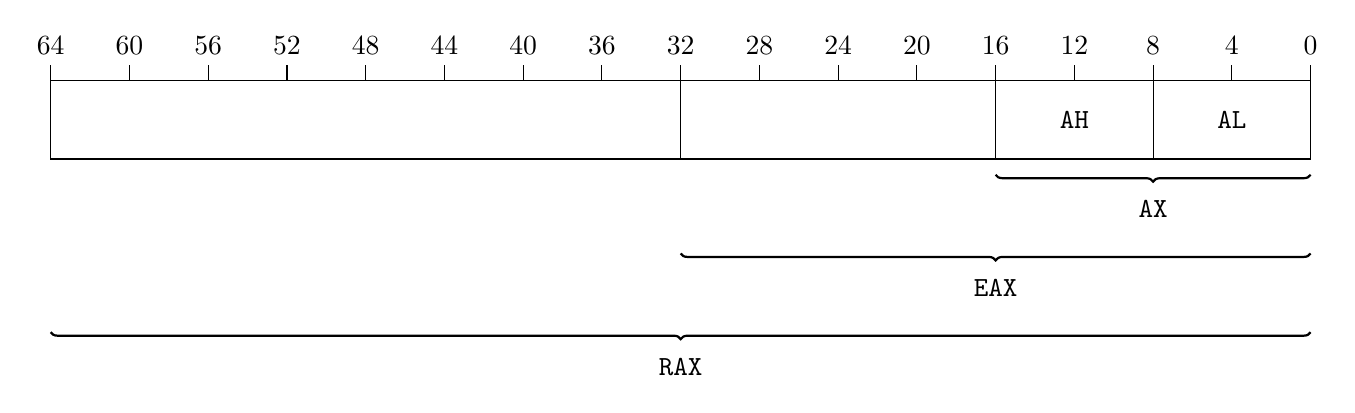
\begin{tikzpicture}
            \foreach \x in {0,...,16} {
                \draw (\x,1) -- (\x,1.2);
                \pgfmathsetmacro\display{64-\x*4}
                \node [above] at (\x,1.2) {\pgfmathprintnumber{\display}};
            }
            \draw (14,0) rectangle (16,1) node[pos=.5] {\texttt{AL}};
            \draw (12,0) rectangle (14,1) node[pos=.5] {\texttt{AH}};
            \draw (8,0) rectangle (12,1) node[pos=.5] {};
            \draw (0,0) rectangle (8,1) node[pos=.5] {};
            \draw [
                thick,
                decorate,
                decoration = {brace, raise=0.2cm}
            ] (16,0) -- (12,0) node[pos=0.5, anchor=north, yshift=-.4cm] {\texttt{AX}};
            \draw [
                thick,
                decorate,
                decoration = {brace, raise=1.2cm}
            ] (16,0) -- (8,0) node[pos=0.5, anchor=north, yshift=-1.4cm] {\texttt{EAX}};
            \draw [
                thick,
                decorate,
                decoration = {brace, raise=2.2cm}
            ] (16,0) -- (0,0) node[pos=0.5, anchor=north, yshift=-2.4cm] {\texttt{RAX}};
        \end{tikzpicture}
    }
    \caption{\texttt{RAX} with its subregisters}
    \label{fig:x86-64-rax-subregs}
\end{figure}


\paragraph{Terminology}
In the following sections we will use the following terminology:
\begin{description}
    \item[Register definition] A write to a register, for example: \texttt{mov eax, 0} defines \texttt{EAX}
    \item[Register usage] An explicit or implicit read from a register, for example: \texttt{mov eax, edx} uses \texttt{EDX}
\end{description}

Instructions may define or use one or more registers implicitly.
\texttt{idiv edi} has an explicit register usage of \texttt{EDI} and an implicit usage of \texttt{EAX}, and is an implicit register definition of \texttt{EDX} and \texttt{EAX}.

\subsubsection{Parameter Discovery}\label{subsubsec:param-discovery}

To detect the parameters of a function, MCTOLL traverses the function's basic blocks via a depth-first search.
Each register usage is then checked.
If the register is one of the argument registers defined in \cref{tab:param-regs} and has not been defined in the current or in all predecessor blocks, it is considered an argument.
Since the \gls{CFG} may contain loops, MCTOLL uses LLVM's \texttt{LoopTraversal} class, which traverses blocks that are part of \gls{CFG} loops twice, to make sure each block's predecessor has been visited at least once.

For each basic block, MCTOLL creates a union of all registers defined in its predecessor blocks.
If two blocks define the same super- but a different subregister, MCTOLL retains the greater one to ensure all incoming values fit the resulting type.

MCTOLL then begins checking the current basic block, iterating over all instructions, and checking each operand.
\begin{itemize}
    \item If the operand is a register use, MCTOLL checks if a predecessor or a previous instruction in the current block defined the super-register.
    If that is not the case, the register should be considered as a potential argument register.
    \item If the operand is a register definition, MCTOLL saves it as defined in the current block.
    In this case, successive instructions and blocks will not consider the register as a potential argument register.
\end{itemize}

Once MCTOLL processed all basic blocks, it checks all potential argument registers.
If the register is a valid argument register, MCTOLL looks up the number and type of the argument and inserts it into the function signature.
If argument $n$ is missing, but argument $n+1$ is defined, it is assumed that argument $n$ was unused and optimized away.
The type of the argument is considered to be \texttt{i64}.

\subsubsection{Type Discovery}\label{subsubsec:type-discovery}

Values passed in general purpose registers are of integer type, with the width of the register as the width of the raised type (\texttt{EDI} $\rightarrow$ \texttt{i32}).
This also means that MCTOLL raises parameters that were initially pointers to \texttt{i64}\footnote{llvm-mctoll only supports raising 64 bit binaries.}.
See~\cref{fig:raised-code-int-args}.

\begin{figure}[htpb]
    \centering
    \begin{subfigure}[t]{.45\textwidth}
        \begin{lstlisting}[language=C]
void test(int, char, char *) {
  ...
}
        \end{lstlisting}
        \caption{Original code}
    \end{subfigure}
    \begin{subfigure}[t]{.45\textwidth}
        \begin{lstlisting}
define dso_local void @test(
  i32 %1, i8  %2, i64 %3) {
...
}
        \end{lstlisting}
        \caption{Raised code}
    \end{subfigure}
    \caption{Discovered arguments passed in general purpose registers}
    \label{fig:raised-code-int-args}
\end{figure}

\subsubsection{Return Type Discovery}\label{subsubsec:return-type-discovery}

To discover the return type of a function, MCTOLL looks at the return blocks and checks if one of the two supported return registers \texttt{RAX} or \texttt{XMM0} has a reaching definition in all of them.
A block is considered a return block if it ends with a return instruction, ignoring padding instructions.
The algorithm to check if all return blocks have a reaching definition of a return register is as follows:
A working list of basic blocks is initialized with the return blocks.
For each block in the working list, its instructions are iterated in reverse order and checked.
\begin{itemize}
    \item If the instruction defines a return register, the return register is also defined for the end of the block.
    Stop iterating over further instructions.
    \item If a call instruction is encountered, stop, as return registers are temporary and not preserved across function calls.
    \item If all instructions have been processed but no return register is defined, add the predecessors of the current block to the working list.
\end{itemize}

The return type of the function is set to that corresponding to the discovered return register.
For functions where no return register has been found, the type is set to \texttt{void}.
Should two return blocks return different-sized integers, the larger one is retained.
This behaviour can be seen in \cref{fig:return-type-detection}.
Since the only return block \texttt{.exit} does not define the return register, we have to look at its predecessors \texttt{.bb.1} and \texttt{.bb.2}.
They define different subregisters, \texttt{EAX} and \texttt{RAX} respectively.
The return type is set to the larger \texttt{i64} instead of \texttt{i32}.

%\begin{algorithmic}
%    \State $workList \gets returnBlocks$
%    \State $visited \gets \emptyset$
%    \While{$worklist \neq \emptyset$}
%        \State $block \gets pop(workList)$
%        \State $visited \gets visited \cup \{block\}$
%        \ForAll{$inst \in reverse(block)$}
%
%        \EndFor
%    \EndWhile
%\end{algorithmic}

\begin{figure}[htpb]
    \centering
    \begin{subfigure}[t]{.45\textwidth}
        \begin{lstlisting}
            test:
              cmp edi, 0
              je .bb.2:
            .bb.1:
              mov eax, 0
              jmp .exit
            .bb.2:
              mov rax, 1
            .exit:
              ret
        \end{lstlisting}
        \caption{Original code}
    \end{subfigure}
    \begin{subfigure}[t]{.45\textwidth}
        \begin{lstlisting}
            define dso_local i64 @test(i32 %1) {
              ; ...
            }
        \end{lstlisting}
        \caption{Raised code with detected return type}
    \end{subfigure}
    \caption{Return type detection example}
    \label{fig:return-type-detection}
\end{figure}

\subsection{Discovering Non-Terminator Instructions}\label{subsec:discovering-non-terminator-instructions}

During the second CFG walk, MCTOLL raises all non-terminator instructions.
To keep track of values stored in registers, a register to \gls{SSA} map is constructed for each function.
This map is updated while raising basic blocks and keeps track of which LLVM value is stored in which register.
\Cref{fig:reg-ssa-map} shows an example of how this map might look while raising a program.

\begin{figure}[htpb]
    \centering
    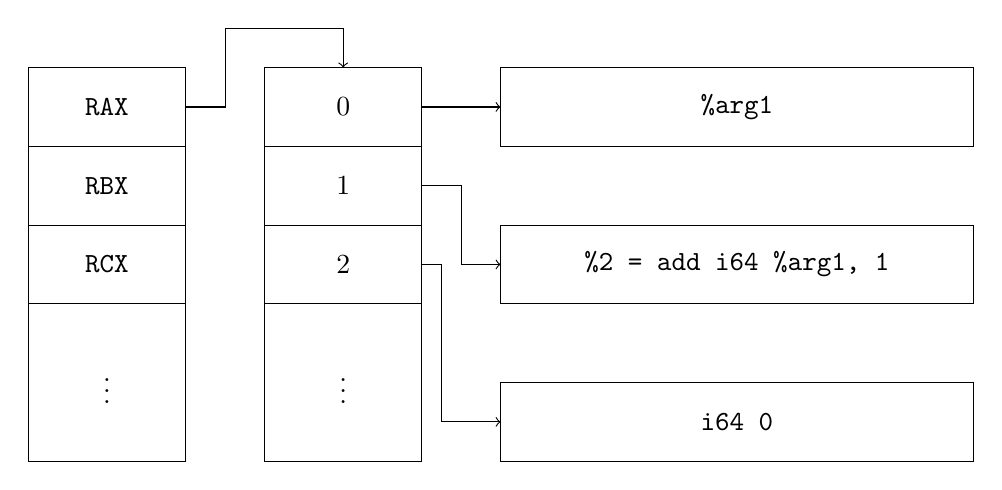
\begin{tikzpicture}
        \draw (0,4) rectangle (2,5) node[pos=.5] (rax) {\texttt{RAX}};
        \draw (0,3) rectangle (2,4) node[pos=.5] (rbx) {\texttt{RBX}};
        \draw (0,2) rectangle (2,3) node[pos=.5] (rcx) {\texttt{RCX}};
        \draw (0,0) rectangle (2,2) node[pos=.5] {\vdots};

        \draw (3,4) rectangle (5,5) node[pos=.5] (bb0) {0};
        \draw (3,3) rectangle (5,4) node[pos=.5] (bb1) {1};
        \draw (3,2) rectangle (5,3) node[pos=.5] (bb2) {2};
        \draw (3,0) rectangle (5,2) node[pos=.5] {\vdots};

        \draw (6,4) rectangle (12,5) node[pos=.5] (val0) {\texttt{\%arg1}};
        \draw (6,2) rectangle (12,3) node[pos=.5] (val1) {\texttt{\%2 = add i64 \%arg1, 1}};
        \draw (6,0) rectangle (12,1) node[pos=.5] (val2) {\texttt{i64 0}};

        \draw[->] (2,4.5) -| (2.5,4.5) |- (4,5.5) -- (4,5);

        \draw[->] (5,4.5) -- (6,4.5);
        \draw[->] (5,3.5) -| (5.5,3.5) |- (6,2.5);
        \draw[->] (5,2.5) -| (5.25,2.5) |- (6,0.5);
    \end{tikzpicture}
    \caption{Register-SSA map keeping track of register values in different blocks}
    \label{fig:reg-ssa-map}
\end{figure}

Each \texttt{MachineInstr} can be translated to zero, one, or more LLVM instructions.
Register moves are not translated to an LLVM instruction, only the register-SSA map is updated.
Instructions such as add operations, where a simple LLVM counterpart exists, translate directly to a single LLVM instruction.
In addition, instructions that implicitly set processor status flags will result in more than one instruction in the raised bitcode.
The value of the processor flags is also stored in the register-SSA map, where successive instructions will be able to access them.
This can be seen in \cref{fig:raised-add-op}, with the initial and updated register-SSA map shown in \cref{fig:raised-add-op-ssa-map}.
If successive instructions do not access generated instructions, LLVM will remove them in its optimization phase when generating code.

\begin{figure}[htpb]
    \centering
    \begin{subfigure}[t]{\textwidth}
        \centering
        \begin{lstlisting}
            add edi, 1
        \end{lstlisting}
        \caption{Original code}
    \end{subfigure}
    \begin{subfigure}[t]{\textwidth}
        \centering
        \begin{lstlisting}
            %EDI = add i32 %arg1, 1
            %0 = call { i32, i1 } @llvm.uadd.with.overflow.i32(i32 %arg1, i32 1)
            %CF = extractvalue { i32, i1 } %0, 1
            ...
        \end{lstlisting}
        \caption{Raised code}
    \end{subfigure}
    \caption[Raised add operation]{Raised add operation}
    \label{fig:raised-add-op}
\end{figure}

\begin{figure}[htpb]
    \begin{subfigure}[t]{0.45\textwidth}
        \centering
        \begin{tikzpicture}[every node/.style={inner sep=10, minimum width=1.5cm}]
            \node[draw] (rdi) {\texttt{RDI}};
            \node[draw, right=of rdi] (bb0-rdi) {0};
            \node[draw, right=of bb0-rdi] (val-rdi) {\texttt{\%arg1}};

            \node[draw, below=of rdi] (cf) {\texttt{CF}};
            \node[draw, right=of cf] (bb0-cf) {0};
            \coordinate[right=of bb0-cf] (val-cf) {};

            \draw[->] (rdi.east) -- (bb0-rdi.west);
            \draw[->] (bb0-rdi.east) -- (val-rdi.west);
            \draw[->] (cf.east) -- (bb0-cf.west);
            \draw[-{Rays}] (bb0-cf.east) -- (val-cf.west);
        \end{tikzpicture}
        \caption{SSA map before raising \texttt{add} instruction}
    \end{subfigure}
    \hfill%
    \begin{subfigure}[t]{0.45\textwidth}
        \centering
        \begin{tikzpicture}[every node/.style={inner sep=10, minimum width=1.5cm}]
            \node[draw] (rdi) {\texttt{RDI}};
            \node[draw, right=of rdi] (bb0-rdi) {0};
            \node[draw, right=of bb0-rdi] (val-rdi) {\texttt{\%EDI}};

            \node[draw, below=of rdi] (cf) {\texttt{CF}};
            \node[draw, right=of cf] (bb0-cf) {0};
            \node[draw, right=of bb0-cf] (val-cf) {\texttt{\%CF}};

            \draw[->] (rdi.east) -- (bb0-rdi.west);
            \draw[->] (bb0-rdi.east) -- (val-rdi.west);
            \draw[->] (cf.east) -- (bb0-cf.west);
            \draw[->] (bb0-cf.east) -- (val-cf.west);
        \end{tikzpicture}
        \caption{SSA map with new value for \texttt{RDI}}
    \end{subfigure}
    \caption{Register-SSA map before and after raising the \texttt{add} operation in \cref{fig:raised-add-op}}
    \label{fig:raised-add-op-ssa-map}
\end{figure}

Terminating instructions such as return or jump instructions are not yet raised in this pass, MCTOLL is gathering information about them to raise them in a subsequent pass.

\subsubsection{Raising Function Calls}\label{subsubsec:raising-function-calls}

If an encountered instruction is a function call, MCTOLL first needs to look up the function prototype.
Function prototypes for external functions need to be passed in the form of header files.
For every argument, MCTOLL looks up the reaching value for the appropriate argument register.
If there is no reaching value, it assumes the argument has been optimized and passes a constant 64 bit integer of zero.

MCTOLL can then construct the LLVM call instruction with the discovered arguments.
If the function is not a \texttt{void} function, MCTOLL updates the register-SSA map for the return register and sets its value to that of the function call.

\paragraph{Vararg Calls}
If the called function is a vararg function, MCTOLL needs to check for additional arguments after the normal arguments.
It does that by iterating over the remaining argument registers and checking for a reaching value for that register.
If a reaching value exists, that value is added to the list of arguments.
Otherwise, the code does not look for further arguments and constructs the function call.

\subsection{Promoting Registers to Stack Slots}\label{subsec:promoting-registers-to-stack-slots}

\begin{figure}[htpb]
    \centering
    \begin{tikzpicture}[
        node distance = 8mm and 12mm,
        block/.style= {draw, font=\ttfamily},
        arr/.style = {semithick, -latex, font=\ttfamily},
    ]
        \node (entry) [block,align=left] {.entry: \\ jz .bb.2};
        \node (bb1) [block,below left=of entry,align=left] {.bb.1:\\mov eax, 1\\jmp .bb.3};
        \draw[arr] (entry) -| node[above] {ZF = 0} (bb1);
        \node (bb2) [block,below right=of entry,align=left] {.bb.2:\\mov eax, 2\\jmp .bb.3};
        \draw[arr] (entry) -| node[above] {ZF = 1} (bb2);
        \node (bb3) [block,below left=of bb2,align=left] {.bb.3:\\mov edi, eax};
        \draw[arr] (bb1) |- (bb3);
        \draw[arr] (bb2) |- (bb3);
    \end{tikzpicture}
    \caption{Control flow graph with a register being defined in multiple predecessors.}
    \label{fig:mctoll-cfg-regs}
\end{figure}

In \cref{fig:mctoll-cfg-regs} we see an example where multiple values reach a block.
In LLVM, there exists a \texttt{phi} instruction, that selects a value depending on which predecessor block was executed before entering the current block.
MCTOLL cannot use this instruction, as not all predecessor are necessarily raised when processing the current block.
As a solution, MCTOLL allocates a stack slot, where the value is stored in all predecessor blocks.
This slot is read in the block where the value is needed.
The code in \cref{fig:mctoll-cfg-regs} is raised to the bitcode shown in \cref{fig:mctoll-stack-promotion}.
If a predecessor block is not raised at the time when the stack slot for a register is created, it is marked as incomplete and processed after all blocks have been translated.

\begin{figure}[htpb]
    \centering
    \begin{lstlisting}
        .entry:
            EAX-STK-LOC = alloca i32, align 4
            ; ...
            br %CF, .bb.1, .bb.2
        .bb.1:
            store i32 1, i32* %EAX-STK-LOC, align 4
            br .bb.3
        .bb.2:
            store i32 2, i32* %EAX-STK-LOC, align 4
            br .bb.3
        .bb.3:
            %EDI = load i32, i32* %EAX-STK-LOC, align 4
    \end{lstlisting}
    \caption{Stack promotion of \texttt{EAX}}
    \label{fig:mctoll-stack-promotion}
\end{figure}

While code with these stack slots is potentially more inefficient, as it will access memory, while \texttt{phi} instructions may be compiled to use registers, LLVM.opt is able to convert these stack accesses to \texttt{phi} nodes, resolving this issue.

\subsection{Peephole Optimizations}\label{subsec:peephole-optimizations}

Peephole optimizations are compiler optimizations that operate on a small set of instructions, analyzing them, and potentially replacing them with a new set of instructions offering better performance~\parencite{10.1145/364995.365000}.
In MCTOLL, peephole optimizations are used to replace certain instruction patterns to make sure the LLVM optimizer is able to optimize them.
One example are memory accesses with an offset as shown in \cref{fig:peephole-opt}.

\begin{figure}[htpb]
    \centering
    \begin{subfigure}[t]{.45\textwidth}
        \begin{lstlisting}
            %1 = ptrtoint i8* %0 to i64
            %2 = add i64 %0, 16
            %3 = inttoptr i64 %0 to i32*
        \end{lstlisting}
        \caption{Original code}
    \end{subfigure}
    \begin{subfigure}[t]{.45\textwidth}
        \begin{lstlisting}
            %1 = getelementptr i8, i8* %0, i64 16
            %2 = bitcast i8* %0 to i32*
        \end{lstlisting}
        \caption{Optimized code}
    \end{subfigure}
    \caption{Example for code optimized by the MCTOLL peephole pass}
    \label{fig:peephole-opt}
\end{figure}


\subsection{Limitations}\label{subsec:limitations}

While MCTOLL allows raising a large set of programs, there are some limitations on what it can do.
Indirect jumps are not supported, as jump targets cannot be detected ahead of time.

Before our contributions to the project, MCTOLL was not able to raise programs from benchmarks such as phoenix-2.0~\parencite{phoenix} and others, as many integer instructions were not supported.
Additionally, almost no SSE instructions were implemented, meaning programs using floating-point arithmetic could not be raised.
In \cref{ch:contributions} we will discuss our contributions to MCTOLL, the instructions that were implemented and bugs that we fixed.
